\section{Metodología}
\label{ch:metodologia}

\subsection{Propuesta de Solución}
\label{sec:propuesta_solucion}
La solución propuesta consiste en el diseño, desarrollo e implementación del Sistema Web de Gestión y Actualización de Datos del Personal del PJETAM, una plataforma web moderna construida sobre el ecosistema de ASP.NET Core que sustituirá por completo al sistema heredado de más de 15 años de antigüedad. El sistema actual, desarrollado originalmente en Visual Basic y ASP.NET Web Forms (el cual se muestra en la Figura \ref{fig:sistema_img}) ha alcanzado el final de su ciclo de vida útil, presentando una severa acumulación de deuda técnica, lentitud extrema debido al procesamiento pesado del estado de las páginas (ViewState), vulnerabilidades críticas en la seguridad de las cuentas y una rigidez estructural que impide agregar nuevas funciones indispensables.

\begin{figure}[htbp]
    \centering
    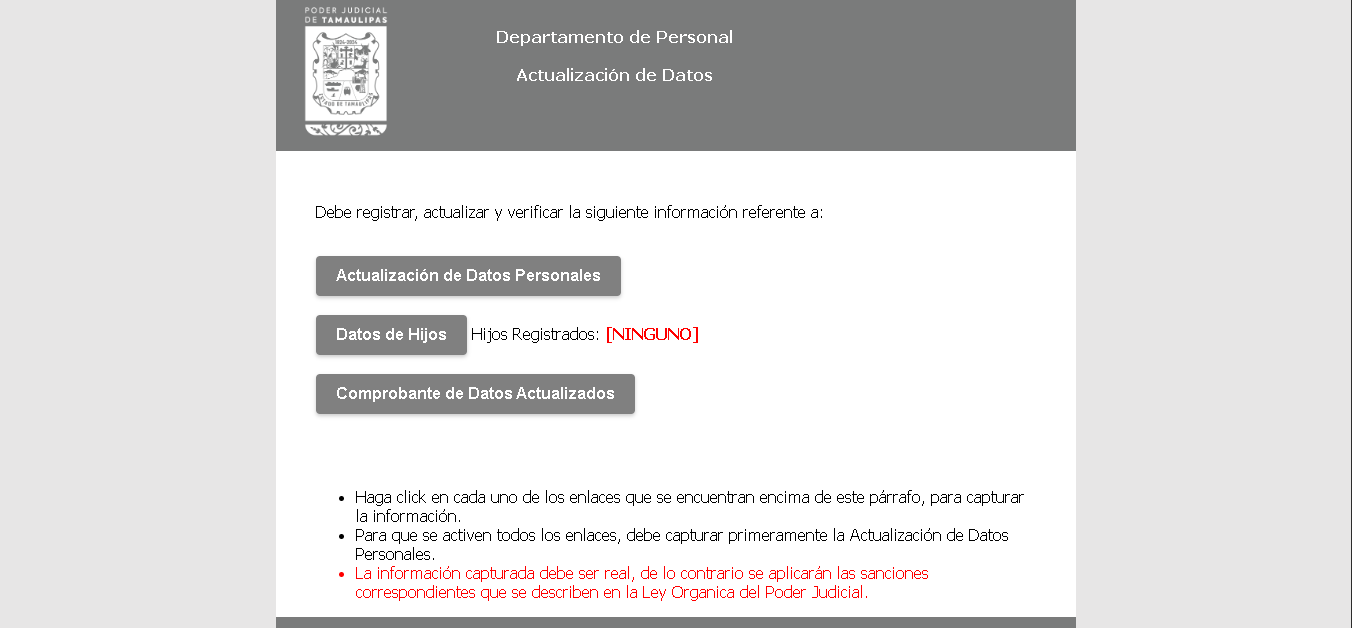
\includegraphics[width=0.9\textwidth]{img/capturasistema.png}
    \caption{Dashboard del Sistema de Actualización de Datos del Personal que se utiliza actualmente en el Poder Judicial de Tamaulipas.}
    \label{fig:sistema_img}
\end{figure}

\subsubsection{Beneficios}
\label{sec:beneficios}

\begin{itemize}
    \item \textbf{Disminución de deuda técnica y mantenibilidad:} Se reemplaza el código monolítico y acoplado del sistema anterior por una estructura limpia basada en la separación de responsabilidades. Esto permitirá que la dirección de informática del Poder Judicial realice modificaciones, correcciones o añada nuevos módulos en el futuro de forma rápida y aislada, sin riesgo de romper otras partes del software.
    \item \textbf{Optimización del rendimiento:} Al eliminar los pesados mecanismos de persistencia en el cliente (ViewState) y los flujos circulares (postbacks) propios de Web Forms, la nueva aplicación web procesará las solicitudes de manera ligera y asíncrona. Esto reducirá drásticamente la carga sobre el servidor del PJETAM y el ancho de banda de la red institucional, garantizando tiempos de respuesta casi inmediatos para los empleados.
    \item \textbf{Fortalecimiento de la seguridad:} La propuesta incluye un esquema de seguridad que remueve los obsoletos proveedores de autenticación del sistema anterior. Se implementará un mecanismo de control de acceso basado en roles (RBAC) y cifrado avanzado de contraseñas para proteger de forma estricta los datos sensibles del personal judicial, asegurando que cada usuario visualice o modifique información exclusivamente de acuerdo con su perfil autorizado.
\end{itemize}

\subsubsection{Recursos Técnicos y de Software}
\label{sec:recursos_tecnicos}

\begin{itemize}
    \item \textbf{Entorno de Desarrollo (IDE):} Microsoft Visual Studio (Edición Enterprise / Community) como plataforma central de codificación.
    \item \textbf{Framework de Desarrollo:} .NET moderno (ASP.NET Core) configurado bajo el patrón MVC.
    \item \textbf{Sistema de Gestión de Base de Datos:} Microsoft SQL Server para la persistencia e integración del repositorio de datos existente. 
    \item \textbf{Herramientas de Mapeo y Migración:} Entity Framework Core integrado mediante la consola de administración de paquetes NuGet.
\end{itemize}

\subsection{Diseño de Interfaz de Usuario}
\label{sec:diseño_interfaz}

\subsubsection{Mockups y Diseños en Figma}
\label{sec:mockups_diseños_figma}
Para empezar con el desarrollo del sistema, primero se definió el diseño de la interfaz del sistema con ayuda de la herramients Figma, ya que esta el útil para crear prototipos interactivos y observar el flujo del sistema antes de empezar a programar.
Para este sistema, no solo se buscó que el diseño fuera más moderno al anterior, sino que se tomó en cuenta el sistema anterior para identificar la información de cada una de la pantallas de los módulos pero también los problemas de usabilidad que surgían.

A partir de esto, se intentó mantener los componentes que ya resultaban familiares para los usuarios, esto para que la transición a este nuevo sistema fuera más sencilla; mientras que para los formularios, se buscó reorganizar la presentación para que los pasos para la navegación fuera menos tediosa.
Durante el diseño también fue importante respetar los lineamientos establecidos en el Manual de Identidad Institucional del Poder Judicial del Estado de Tamaulipas. Se utilizaron los colores oficiales de la institución, la tipografía y el logotipo autorizados, manteniendo así una nueva interfaz moderna pero corporativa y profesional.

\paragraph{Pantalla de Inicio de Sesión} ~\\
\label{sec:inicio_sesion}El diseño para la pantalla de inicio de sesión del anterior sistema tenía una aspecto tradicional y con pocos elementos visuales, por lo que se buscó un diseño más moderno y atractivo, pero sin perder la formalidad.
Se decidió centrar el formulario de autenticación en una interfaz sencilla con los campos de usuario y contraseña. 

De esta manera, se evitan elementos innecesarios que podrían distraer al personal; también se agregó el logotipo institucional y los colores definidos por el Manual de Identidad del Poder Judicial.
El objetivo principal de esta pantalla es reducir la complejidad, y que así el acceso al sistema pueda ser rápido e intuitivo, sin importar si el usuario es nuevo o ya tiene experiencia.

\begin{figure}[H]
    \centering
    \begin{subfigure}[b]{0.45\textwidth}
        
\includegraphics[width=\textwidth]{img/mockup1.png}
        \caption{Mockup del login.}
        \label{fig:mockup_login}
    \end{subfigure}
    \hfill
    \begin{subfigure}[b]{0.45\textwidth}
        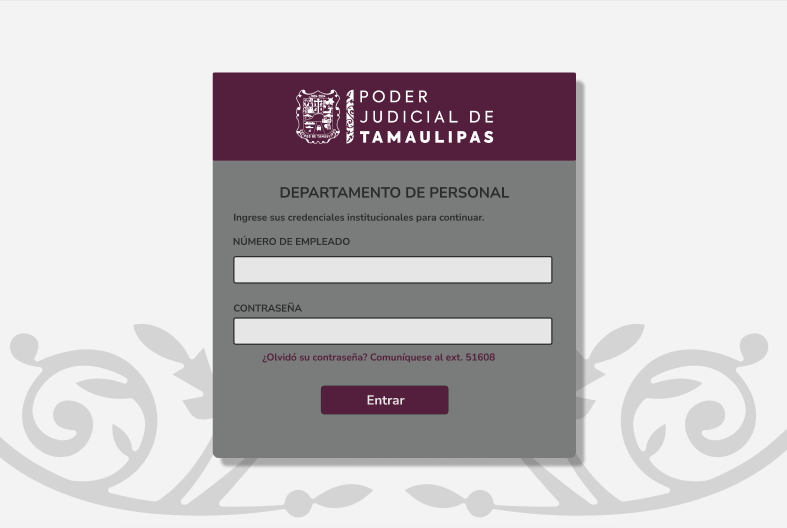
\includegraphics[width=\textwidth]{img/figma1.png}
        \caption{Prototipo de login en Figma.}
        \label{fig:figma_login}
    \end{subfigure}
    \caption{Mockup y prototipo de la pantalla de inicio de sesión del sistema.}
    \label{fig:login_figuras}
\end{figure}

\paragraph{Dashboard} ~\\
\label{sec:dashboard}

\paragraph{Formulario de Datos Personales} ~\\
\label{sec:formulario_datos}

\paragraph{Formulario de Datos de Hijos} ~\\
\label{sec:formulario_hijos}

\paragraph{Comprobante} ~\\
\label{sec:comprobante}



\subsection{Desarrollo del Sistema}
\label{sec:desarrollo_sistema}

\subsubsection{Diagramas de Casos de Uso}
\label{sec:diagramas_casos_uso}

\subsubsection{Diagramas de Bases de Datos}
\label{sec:diagramas_bases_datos}

\subsubsection{Diagramas de Actividades}
\label{sec:diagramas_actividades}

\subsubsection{Diagramas de Secuencia}
\label{sec:diagramas_secuencia}